% !TEX root = ../master-thesis.tex

Achieving single-site resolution in quantum gas microscopy is crucial for experiments probing quantum many-body phenomena. Conventional imaging techniques typically rely on high numerical aperture (N.A.) objectives to directly resolve atomic distributions in optical lattices. However, even with advanced optics, direct imaging is often limited by the fundamental diffraction limit and the intrinsic diffusion of atoms during photon scattering. In particular, for lattice spacings on the order of a micrometer or below—such as the bow-tie lattice spacing of 0.75$\mu$m used in our experiment—direct imaging becomes impractical due to both optical resolution limits and momentum kicks received by atoms from resonant imaging light, causing significant spatial diffusion.

To overcome these limitations, we utilize the technique of matter-wave magnification (MWM), which enables significant enlargement of the spatial distribution of atoms prior to the imaging process \cite{huang_construction_2024}. MWM operates by carefully engineering the evolution of atomic ensembles through controlled harmonic potentials. This method enlarges spatial patterns coherently, thus facilitating the detection of atomic distributions with improved resolution.

The principle underlying MWM can be understood from the perspective of phase-space dynamics. Consider atoms initially confined near the turning points of a harmonic potential with frequency $\omega_1$. After evolving for a quarter of the harmonic period $T_1/4=\pi/2\omega_1$, their spatial distribution transforms entirely into momentum space. Subsequently, atoms are subjected to a second, weaker harmonic potential characterized by frequency $\omega_2$ for another quarter period $T_2/4=\pi/2\omega_2$. During this second stage, the momentum-space distribution converts back into real space, resulting in magnification by a factor given by the ratio $\omega_1/\omega_2$ \cite{huang_construction_2024}. From the viewpoint of the Schrödinger equation, each evolution step corresponding to a quarter period in a harmonic potential functions as a Fourier transformation, converting between position and momentum space representations.


\begin{figure}
    \centering
    \addletter{130}{a}
    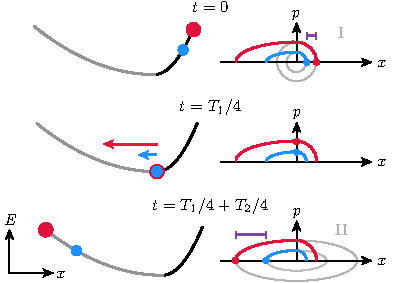
\includegraphics{fig-ai/mwm-scheme.pdf}
    \addletter{130}{b}
    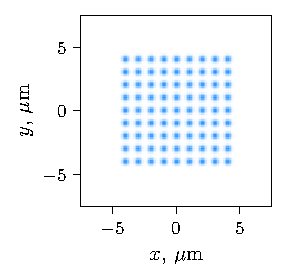
\includegraphics{fig-py/mwm-1.pdf}
    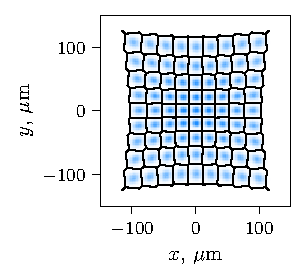
\includegraphics{fig-py/mwm-2.pdf}
    \caption{
    \textbf{Matter-wave magnification scheme and ROI adaptation.}
    (a) Conceptual illustration of matter-wave magnification: atoms initially localized at the slope of a harmonic potential with frequency $\omega_1$ roll towards the center during a quarter period. Subsequent expansion in a shallower harmonic potential with frequency $\omega_2$ increases their spatial separation by the factor $\omega_1/\omega_2$.
    (b) Initial atom distribution (left) and magnified pattern after propagation (right), demonstrating distortion due to anharmonicities. Voronoi diagrams adapt the regions of interest (ROI) to these distorted patterns, improving atom detection fidelity.
    }
    \label{fig:mwm}
\end{figure}

However, practical implementation of MWM faces several challenges, notably potential anharmonicities that cause distortions of the magnified atomic pattern. These distortions necessitate adaptive methods for defining regions of interest (ROI) to ensure accurate atom detection. In this work, the application of Voronoi diagrams was introduced to adjust ROI based on actual atomic distributions post-magnification, thus potentially enhancing detection fidelity.

% The following sections detail the numerical methods developed and applied within this thesis to simulate the wavefunction dynamics and classical trajectories of atoms undergoing MWM. We discuss explicitly our numerical approach combining Monte Carlo simulations with the Runge-Kutta 4th order method (RK4), alongside quantum wavefunction evolution techniques via the split-step method. We further elaborate on how the Voronoi-based ROI adaptation provides a robust and efficient approach to handle the inherent spatial distortions introduced by anharmonic potentials.




% MWM был подробно разобран в контексте нашего эксперимента в \cite{huang_construction_2024}. В рамках этой работы хочу коснуться моментов которые выполнялись в рамках этой работы: наработки в численном моделировани и особенности от MWM в imaging. В контексте численного моделирования это monte carlo with RK4 for 2D MWM with gpu support, split step method for Scrodinger equation in 1D and 2D (нет нужны в многочастичности, так как частицы в MWM будут в точке невзаимодействия, так что хорошо описываются классически. Но можно и квантово, но с точки зрения средней плотности всё ещё достаточно сумм |psi|^2 а вот для относительного положения уже пригодится кванты если важна фермионность как в примере на рисунке. В целом можно и для сколько угодно частиц строить такие штуки с DPP \red{см Аппендикс}) Так как MWM может вызывать некоторые distortion регулярной решётки, то возникает вопрос выбора ROI для каждого твизера, естественным решением которого будут диаграммы Вороного. 

% Position and Momentum Correlations \cite{bergschneider_experimental_2019}

% Про производительность моего 2D monte carlo кода: 4s (A100 for 1k rk4 steps and 1.6e6 particles)





\begin{figure}
    \centering
    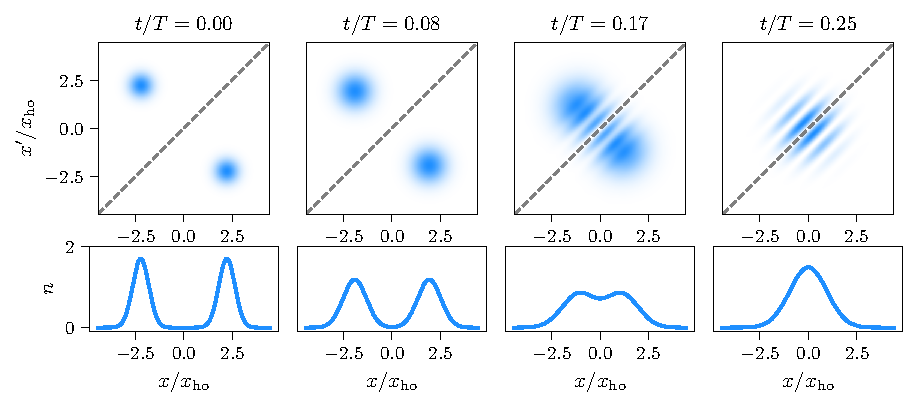
\includegraphics{fig-py/interference.pdf}
    \caption{
        \textbf{Two-fermion dynamics in a 1D harmonic trap: quantum statistics.}
        Top row: Time evolution of the two-particle correlation function $P_2(x,x')$ for two fermions in a harmonic potential. The characteristic anti-bunching dip along the diagonal reflects fermionic quantum statistics, contrasting the bunching peak expected for bosons. Bottom row: Corresponding single-particle density profiles $n(x)$, which remain indistinguishable from the bosonic case, highlighting the necessity of two-particle correlations to probe quantum statistics.
        }
    \label{fig:interference}
\end{figure}

